\newpage

\section{Trigonometrie}
\subsection{Gradmass, Bogenmass}
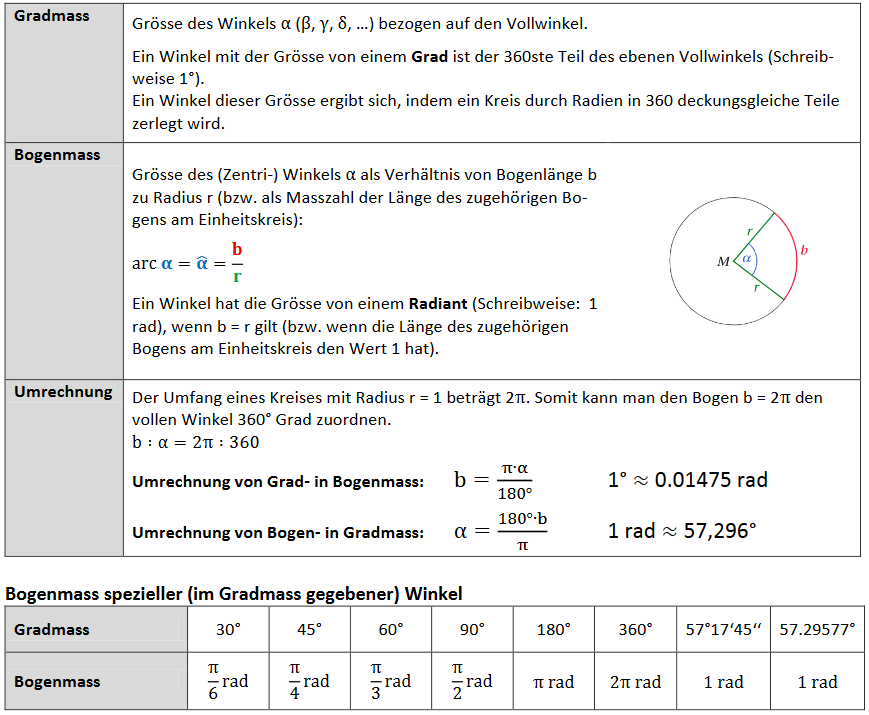
\includegraphics[scale=0.7]{gradmass.PNG}
\subsection{Trigonometrische Funktionen am rechtwinkligen Dreieck}
\subsubsection{Sinus, Kosekans}
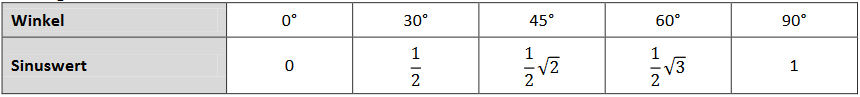
\includegraphics[scale=0.7]{sinkan1.PNG}

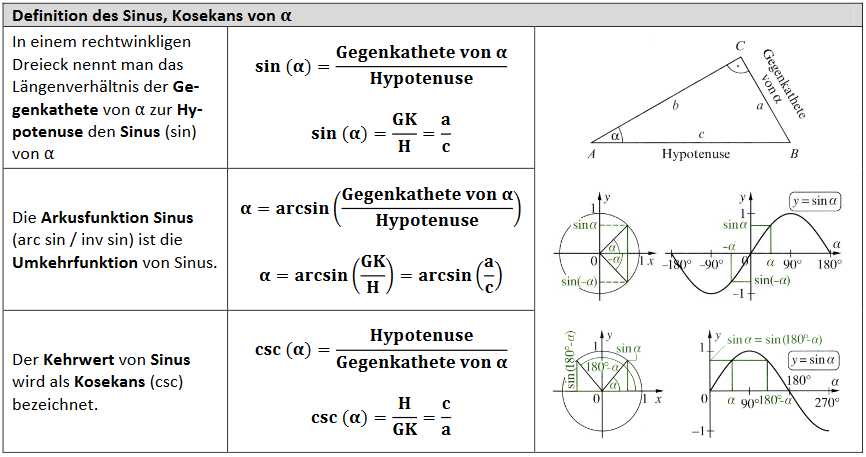
\includegraphics[scale=0.7]{sinkan2.PNG}
\subsubsection{Kosinus, Sekans}
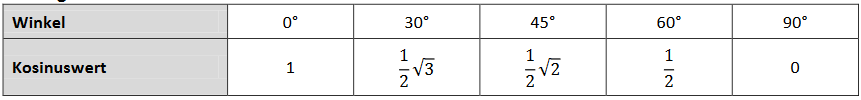
\includegraphics[scale=0.7]{kossek1.PNG}

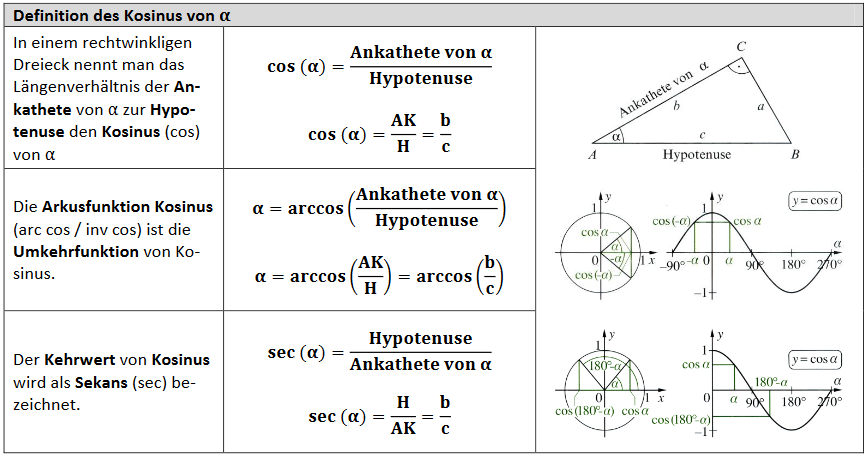
\includegraphics[scale=0.7]{kossek2.PNG}
\subsubsection{Tangens, Kotangens}
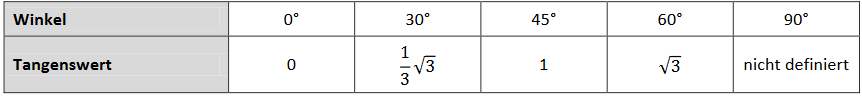
\includegraphics[scale=0.7]{tanko1.PNG}

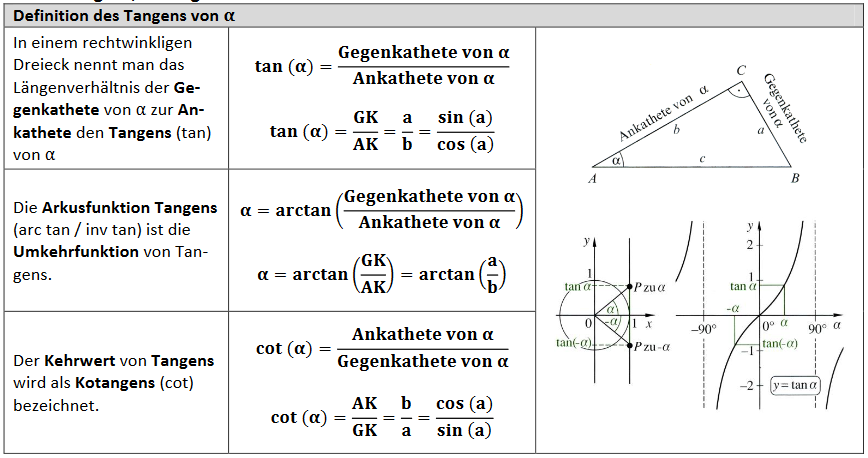
\includegraphics[scale=0.7]{tanko2.PNG}

\subsubsection{Sinus- Kosinus- und Tangensfunktion am rechtwinkligen Dreieck}
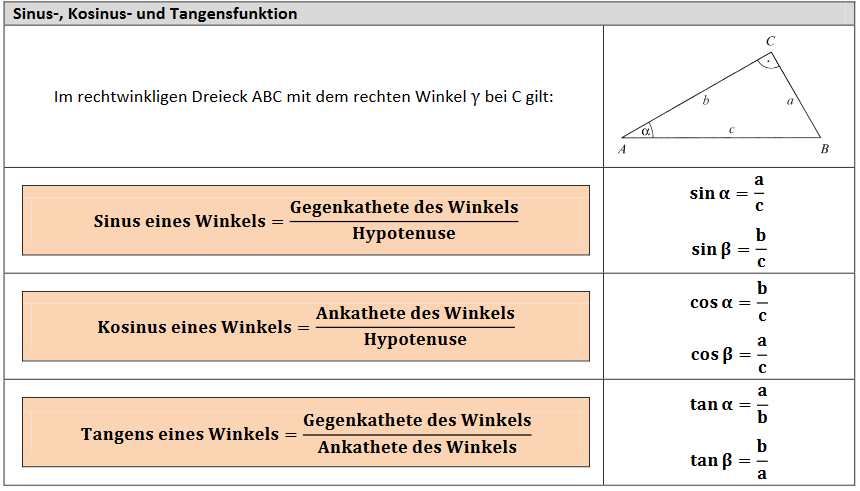
\includegraphics[scale=0.7]{sinkota.PNG}

\newpage{}


\subsection{Trigonometrische Funktionen am schiefwinkligen Dreieck}
\subsubsection{Kosinussatz}
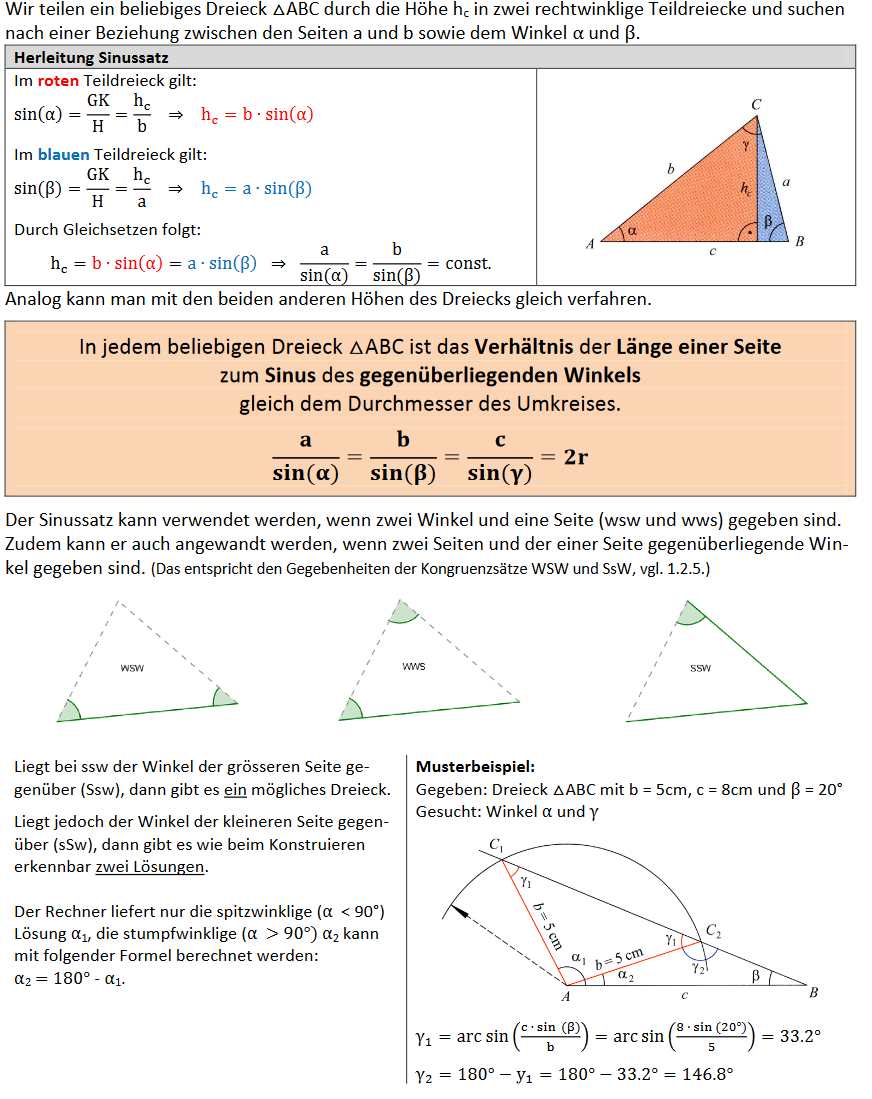
\includegraphics[scale=0.7]{sinussatz.PNG}
\subsubsection{Sinussatz}
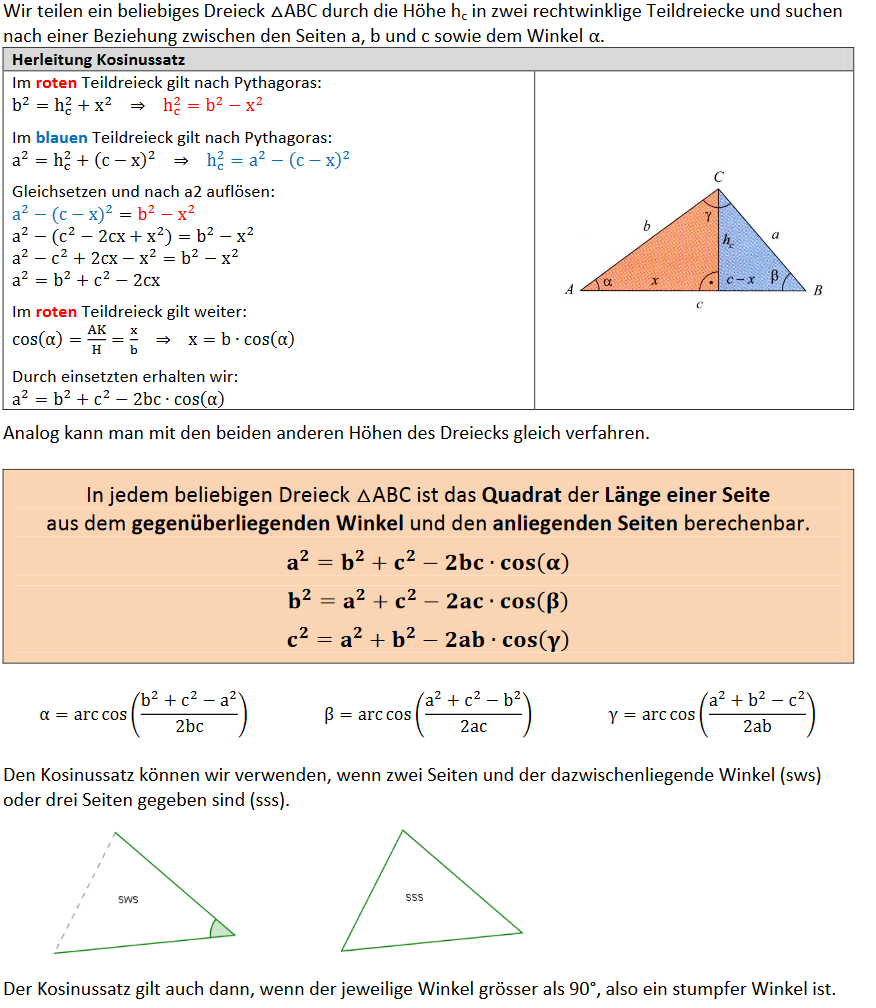
\includegraphics[scale=0.7]{kosinussatz.PNG}

\subsubsection{Flaechensatz}
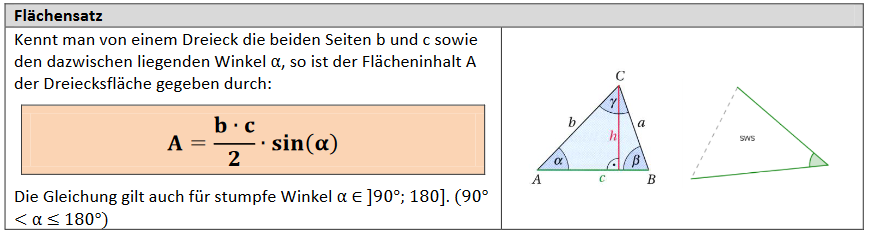
\includegraphics[scale=0.7]{flaechensatz.PNG}
\subsubsection{Berechnung am Kreissektor (auch Kreisausschnitt)}
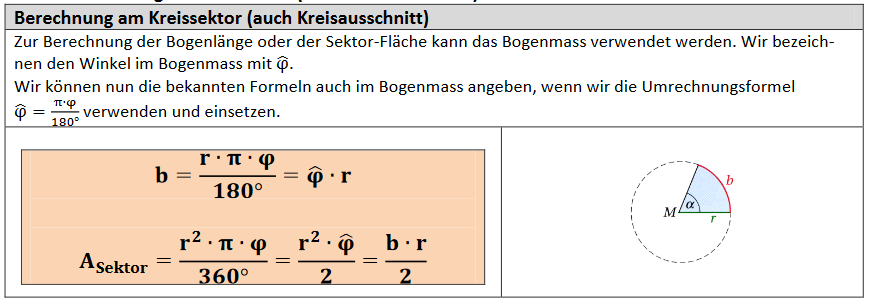
\includegraphics[scale=0.7]{kreissektor.PNG}
\subsubsection{Kreissegment (auch Kreisabschnitt)}
\includegraphics[scale=0.7]{kreissegment.PNG}



\subsection{Einheitskreis}
\subsubsection{Definition}
Der Einheitskreis ist ein Kreis um den Koordinatenursprung mit dem Radius r = 1 Laengeneinheit.
\subsubsection{Sinus- und Kosinusfunktion}
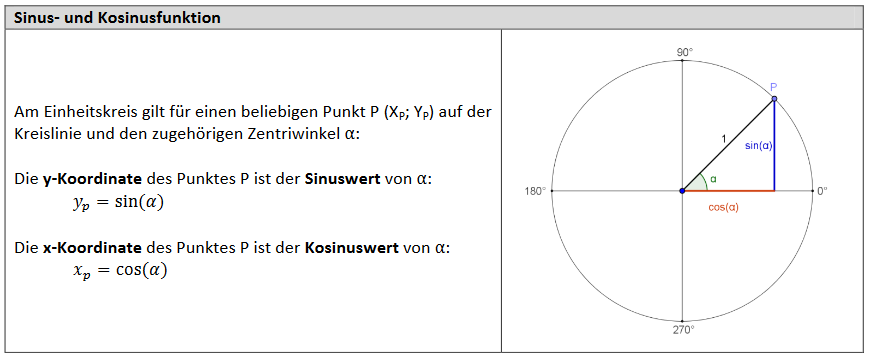
\includegraphics[scale=0.7]{einheitskreis1.PNG}
\subsubsection{Tangentsfunktion}
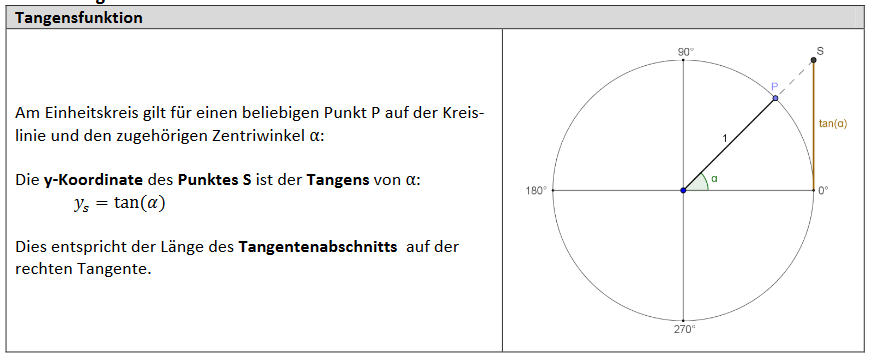
\includegraphics[scale=0.7]{einheitskreis2.PNG}
\subsubsection{Beziehungen zwischen den Winkelfunktionen (Phytagoras am Einheitskreis)}
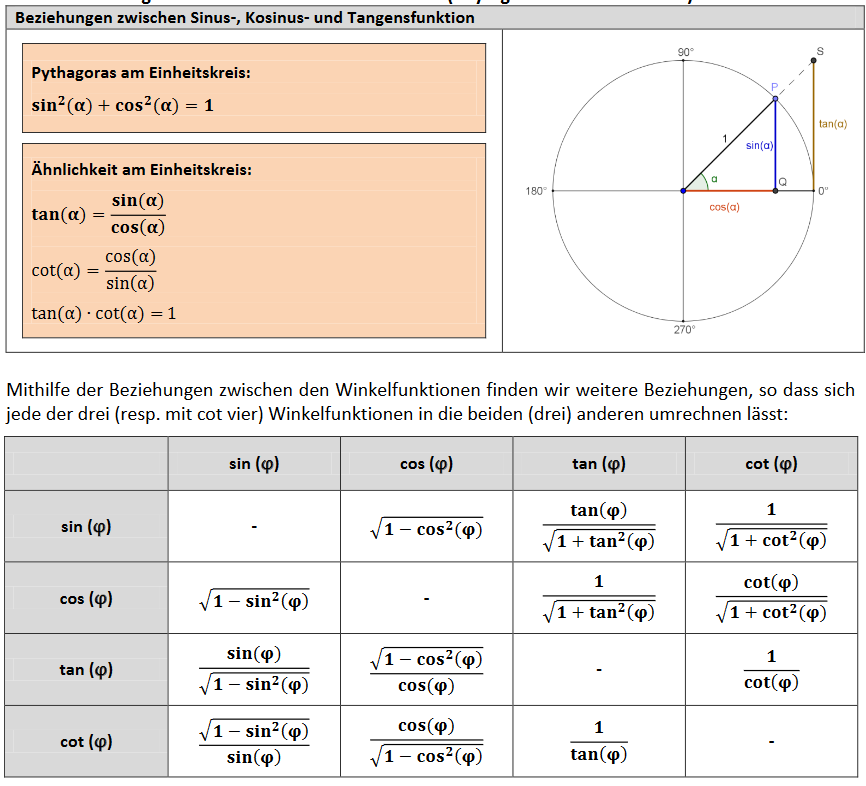
\includegraphics[scale=0.7]{einheitskreis3.PNG}
\subsubsection{Vorzeichen der Trigonometrischen Funktionen}
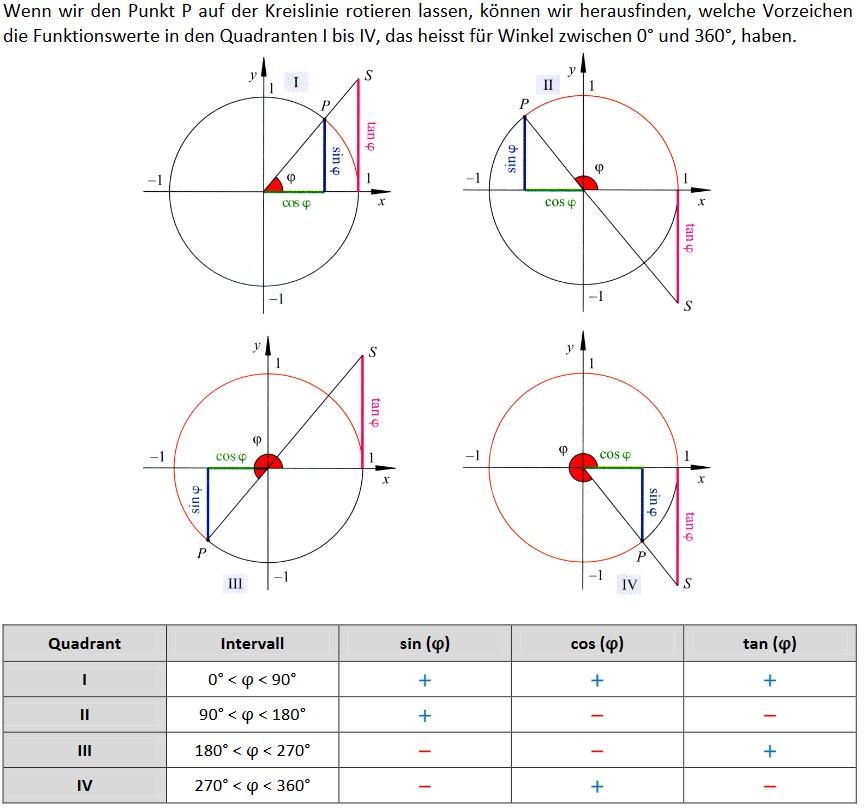
\includegraphics[scale=0.7]{einheitskreis4.PNG}

\subsection{Eigenschaften der Funktionen}
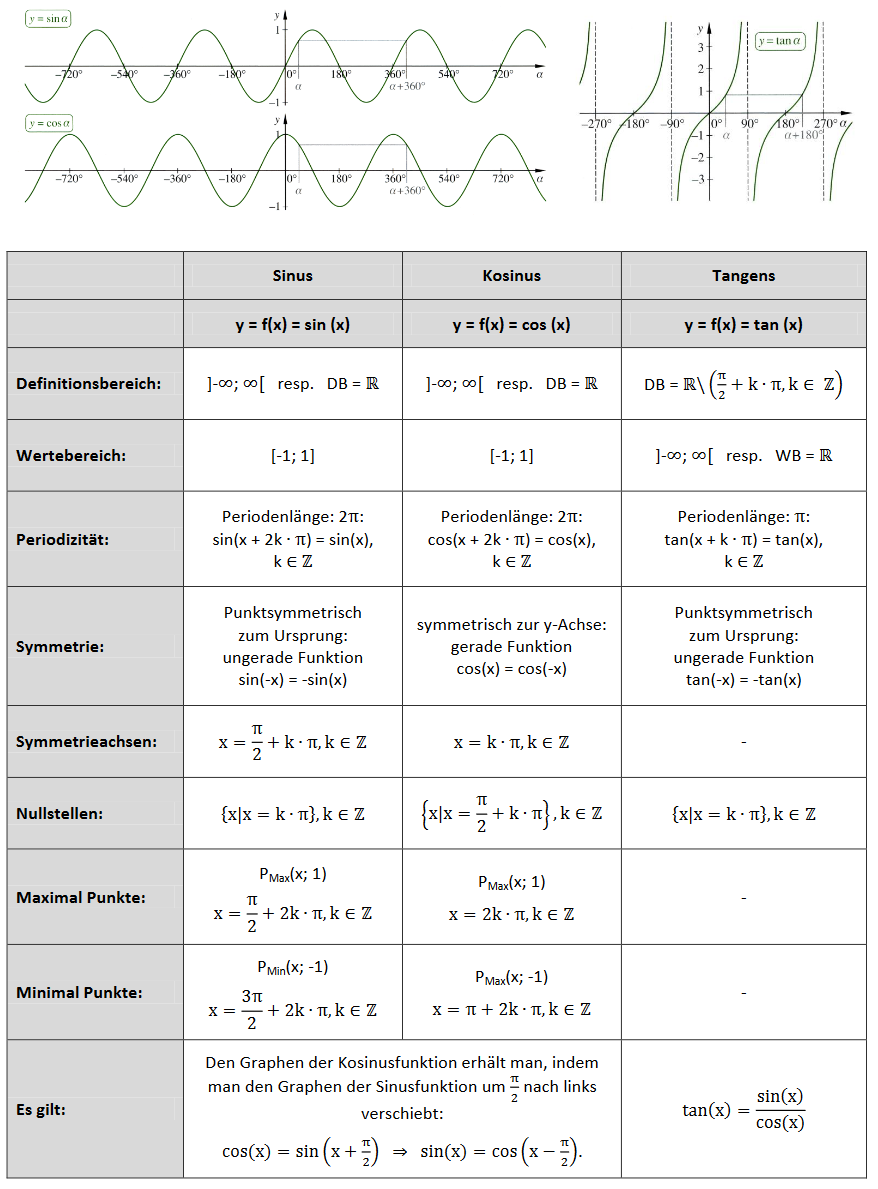
\includegraphics[scale=0.7]{trigfunktionen.PNG}

\subsection{Transformation der Sinusfunktion}
\subsubsection{Parameter a: Strecken. Stauchen auf der y-Achse (Amplitude)}
$y = a \cdot \sin(x)$ wobei $a \in \mathbb{R}\setminus0$ \\

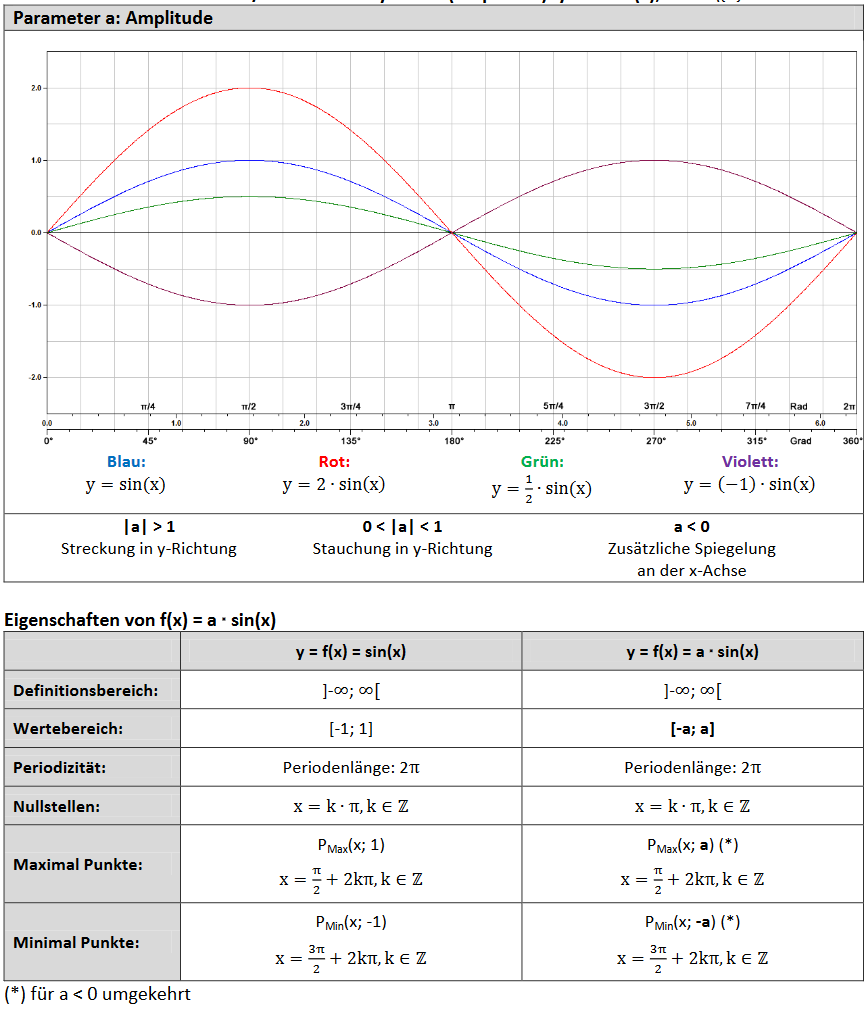
\includegraphics[scale=0.8]{sinus1.PNG}
\subsubsection{Parameter b: Strecken. Stauchen auf der x-Achse}
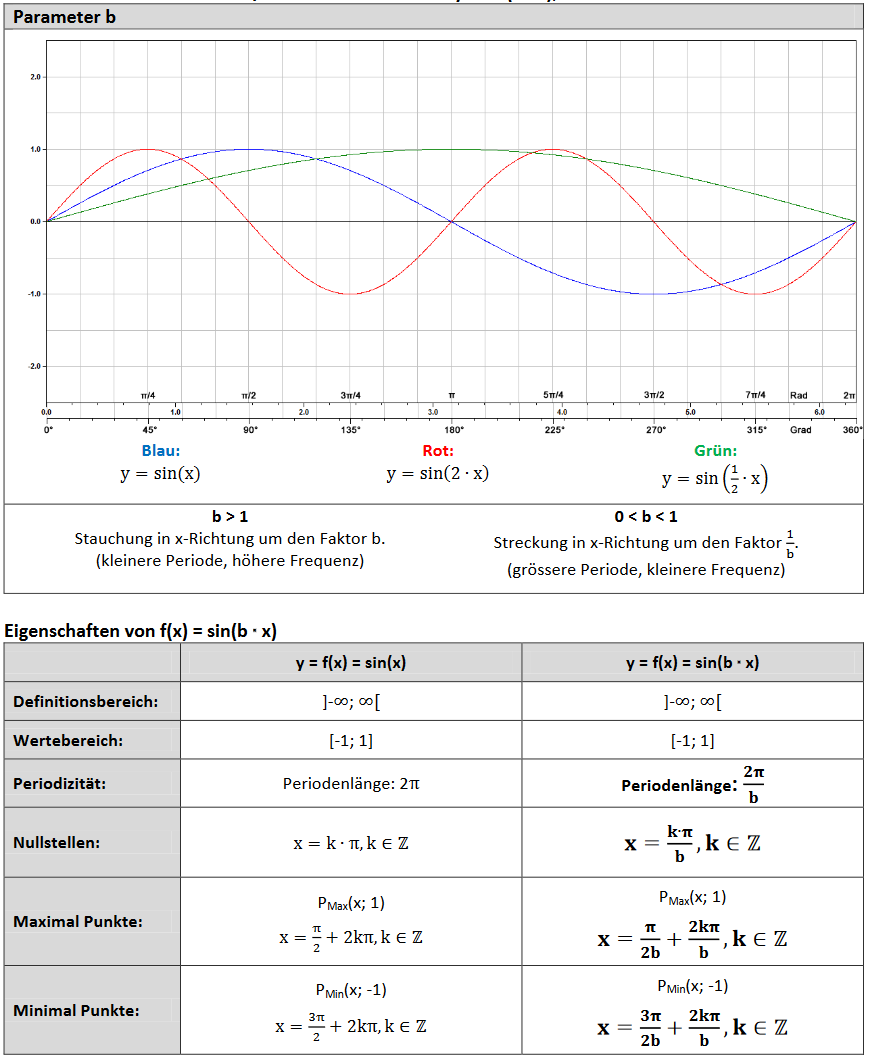
\includegraphics[scale=0.8 ]{sinus2.PNG}

\newpage{}
\section{Goniometrie}
\subsection{Grundlagen}
\subsubsection{Beziehungen}
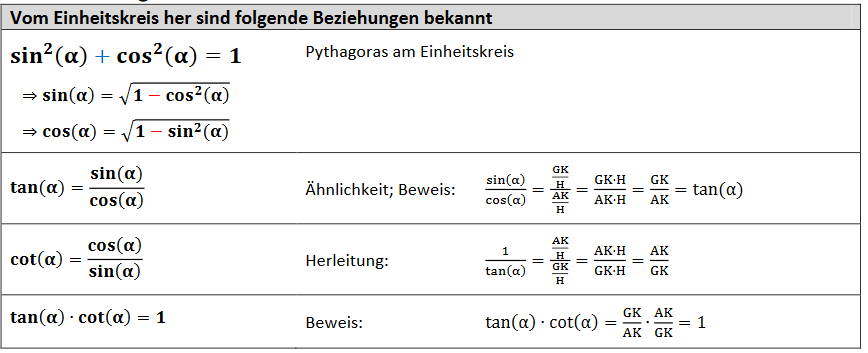
\includegraphics[scale=0.7]{gon1.PNG}

\subsubsection{Additionstheoreme}
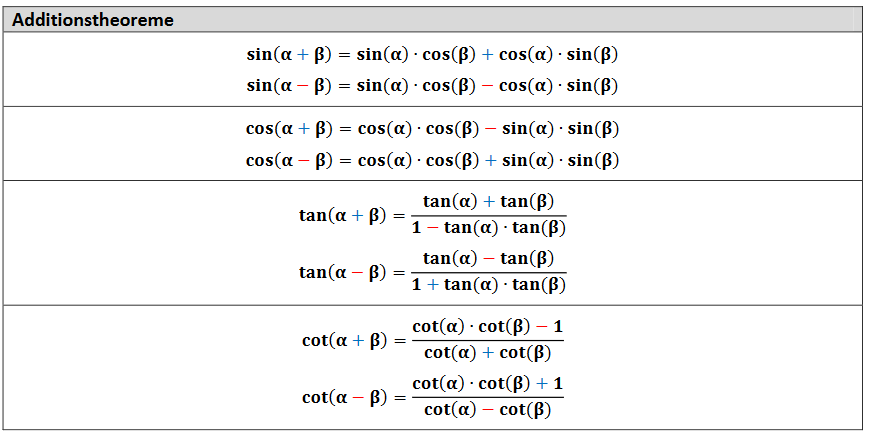
\includegraphics[scale=0.7]{gon2.PNG}

\subsubsection{Winkelfunktionen des doppelten Winkels}
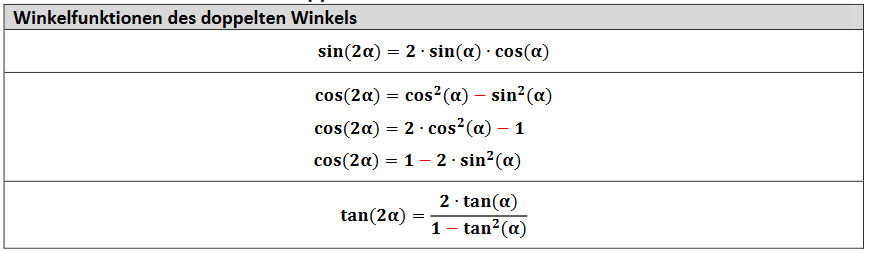
\includegraphics[scale=0.7]{gon3.PNG}

\subsubsection{Winkelfunktionen des dreifachen Winkels}
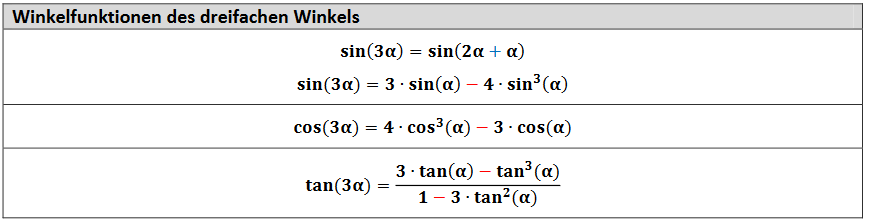
\includegraphics[scale=0.7]{gon4.PNG}

\subsubsection{Winkelfunktionen des halben Winkels}
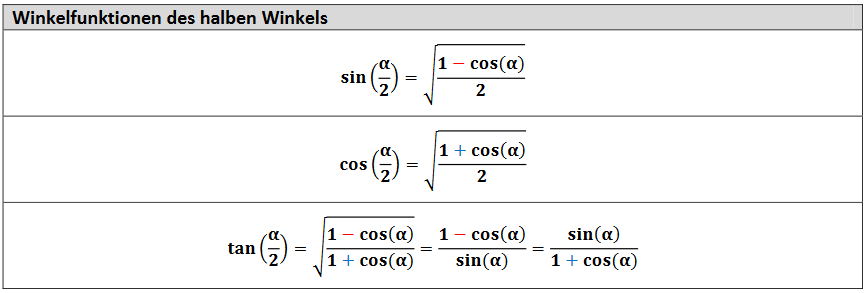
\includegraphics[scale=0.7]{gon5.PNG}

\section{Vektorgeometrie}
\textbf{Vektor:}

Ein Vektor ist festgelegt durch eine Laenge (Groesse) und eine Richtung.

\textbf{Freie Vektoren: }
Sie beschreiben Merkmale,
bei denen es nur auf Grösse und Richtung ankommt

\textbf{Ortsvektoren:}
Sie beschreiben Merkmale,
bei denen es auf Grösse, Richtung und Anfangspunkt ankommt


\subsection{Grundrechenarten}
\subsubsection{Addition von Vektoren}

\subsubsection{Subtraktion von Vektoren}

\subsubsection{Multiplikation mit einer Zahl}

\subsubsection{Skalarprodukt}

\subsubsection{Vektorprodukt}



\newpage{}
